%% В этот файл не предполагается вносить изменения

% В этом файле следует указать информацию о себе
% и выполняемой работе.

\documentclass [fontsize=14pt, paper=a4, pagesize, DIV=calc]%
{scrreprt}
% ВНИМАНИЕ! Для использования глав поменять
% scrartcl на scrreprt

% Здесь ничего не менять
\usepackage [T2A] {fontenc}   % Кириллица в PDF файле
\usepackage [utf8] {inputenc} % Кодировка текста: utf-8
\usepackage [main=english, finnish, russian] {babel} % Переносы, лигатуры

%%%%%%%%%%%%%%%%%%%%%%%%%%%%%%%%%%%%%%%%%%%%%%%%%%%%%%%%%%%%%%%%%%%%%%%%
% Создание макроса управления элементами, специфичными
% для вида работы (курс., бак., маг.)
% Здесь ничего не менять:
\usepackage{ifthen}
\newcounter{worktype}
\newcommand{\typeOfWork}[1]
{
	\setcounter{worktype}{#1}
}

% ВНИМАНИЕ!
% Укажите тип работы: 0 - курсовая, 1 - бак., 2 - маг.,
% 3 - бакалаврская с главами.
\typeOfWork{2}
% Считается, что курсовая и бак. бьются на разделы (section) и
% подразделы (subsection), а маг. — на главы (chapter), разделы и
%  подразделы. Если хочется,
% чтобы бак. была с главами (например, если она большая),
% надо выбрать опцию 3.

% Если при выборе 2 или 3 вы забудете поменять класс
% документа на scrreprt (см. выше, в самом начале),
% то получите ошибку:
% ./aux/appearance.tex:52: Package scrbase Error: unknown option ` chapterprefix=

%%%%%%%%%%%%%%%%%%%%%%%%%%%%%%%%%%%%%%%%%%%%%%%%%%%%%%%%%%%%%%%%%%%%%%%%
% Информация об авторе и работе для титульной страницы

\usepackage {titling}

% Имя автора в именительном падеже (для маг.)
\newcommand {\me}{%
М.\,И.~Глухова%
}

% Имя автора в родительном падеже (для курсовой и бак.)
\newcommand {\byme}{%
М.\,И.~Глуховой%
}

% Научный руководитель
\newcommand{\supervisor}%
{профессор, доктор физико-математических наук В. С. Пилиди, \\Associate Professor Arto Kaarna}

% идентифицируем пол (только для курсовой и бак.)
\newcommand{\bystudent}{
Студентки % Для курсовой: с большой буквы
}

% Год публикации
\date{2017}

% Название работы
\title{Инструменты обеспечения повторяемых сборок \\для свободного программного обеспечения}

% Кафедра
%

\newcommand {\direction} {%
Направление подготовки\\02.\ifthenelse{\value{worktype} = 2}{04}{03}.02 ---
Фундаментальная информатика\\и информационные технологии%
}

% Нумерация списков: можно при необходимести
% изменять вид нумерации (например, добавлять правую скобку).
% По умолчанию буду списки вида:
% 1.
% 2.
% Изменять вид нумерации можно в начале нумерации:
% \begin{enumerate}[1)] (В квадратных скобках указан желаемый вид)
\usepackage[shortlabels]{enumitem}
                    \setlist[enumerate, 1]{1.}

% Гиперссылки: настройте внешний вид ссылок
\usepackage%
[pdftex,unicode,pdfborder={0 0 0},draft=false,%backref=page,
    hidelinks, % убрать, если хочется видеть ссылки: это
               % удобно в PDF файле, но не должно появиться на печати
    bookmarks=true,bookmarksnumbered=false,bookmarksopen=false]%
{hyperref}


\usepackage {amsmath}      % Больше математики
\usepackage {amssymb}
\usepackage {textcase}     % Преобразование к верхнему регистру
\usepackage {indentfirst}  % Красная строка первого абзаца в разделе

\usepackage {fancyvrb}     % Листинги: определяем своё окружение Verb
\DefineVerbatimEnvironment% с уменьшенным шрифтом
	{Verb}{Verbatim}
	{fontsize=\small}

% Вставка рисунков
\usepackage {graphicx}

% Общее оформление
% ----------------------------------------------------------------
% Настройка внешнего вида

%%% Шрифты

% если закомментировать всё — консервативная гарнитура Computer Modern
\usepackage{paratype} % профессиональные свободные шрифты
%\usepackage {droid}  % неплохие свободные шрифты от Google
%\usepackage{mathptmx}
%\usepackage {mmasym}
%\usepackage {psfonts}
%\usepackage{lmodern}
%var1: lh additions for bold concrete fonts
%\usepackage{lh-t2axccr}
%var2: the package below could be covered with fd-files
%\usepackage{lh-t2accr}
%\usepackage {pscyr}
\usepackage{lastpage}   % page count

% Геометрия текста

\usepackage{setspace}       % Межстрочный интервал
\onehalfspacing

\newlength\MyIndent
\setlength\MyIndent{1.25cm}
\setlength{\parindent}{\MyIndent} % Абзацный отступ
\frenchspacing            % Отключение лишних отступов после точек
\KOMAoptions{%
    DIV=calc,         % Пересчёт геометрии
    numbers=endperiod % точки после номеров разделов
}

                            % Консервативный вариант:
%\usepackage                % ручное задание геометрии
%[%                         % (не рекомендуется в проф. типографии)
%  margin = 2.5cm,
  %includefoot,
  %footskip = 1cm
%] %
%  {geometry}

%%% Заголовки


\ifthenelse{{\value{worktype} > 1}}{%
  \KOMAoptions{%
      headings=normal,   % размеры заголовков поменьше стандартных
      %chapterprefix=true,% Печатать слово Глава
      appendixprefix=true% Печатать слово Приложение
  }
}{% Печатать слово Приложение даже если нет глав
  \newcommand*{\appendixmore}{%
    \renewcommand*{\sectionformat}{%
    \appendixname~\thesection\autodot\enskip}
    \renewcommand*{\sectionmarkformat}{%
      \appendixname~\thesection\autodot\enskip}
  }
}

% шрифт для оформления глав и названия содержания
\newcommand{\SuperFont}{\Large\sffamily\bfseries}

% Заголовок главы
\ifthenelse{\value{worktype} > 1}{%
\renewcommand{\SuperFont}{\Large\normalfont\sffamily}
\newcommand{\CentSuperFont}{\centering\SuperFont}
\usepackage{fncychap}
\ChNameVar{\SuperFont}
\ChNumVar{\CentSuperFont}
\ChTitleVar{\CentSuperFont}
\ChNameUpperCase
\ChTitleUpperCase
}

% Заголовок (под)раздела с абзацного отступа
\addtokomafont{sectioning}{\hspace{\MyIndent}}

\renewcommand*{\captionformat}{~---~}
\renewcommand*{\figureformat}{Figure~\thefigure}


%%% Оглавление
\usepackage{tocloft}

% шрифт и положение заголовка
\ifthenelse{\value{worktype} > 1}{%
\renewcommand{\cfttoctitlefont}{\hfil\SuperFont\MakeUppercase}
}{
\renewcommand{\cfttoctitlefont}{\hfil\SuperFont}
}

% слово Глава
\usepackage{calc}
\ifthenelse{\value{worktype} > 1}{%
\renewcommand{\cftchappresnum}{Chapter }
\addtolength{\cftchapnumwidth}{\widthof{Chapter }}
}

% Очищаем оформление названий старших элементов в оглавлении
\ifthenelse{\value{worktype} > 1}{%
\renewcommand{\cftchapfont}{}
\renewcommand{\cftchappagefont}{}
}{
\renewcommand{\cftsecfont}{}
\renewcommand{\cftsecpagefont}{}
}

% Точки после верхних элементов оглавления
\renewcommand{\cftsecdotsep}{\cftdotsep}
%\newcommand{\cftchapdotsep}{\cftdotsep}

\ifthenelse{\value{worktype} > 1}{%
    \renewcommand{\cftchapaftersnum}{.}
}{}
\renewcommand{\cftsecaftersnum}{.}
\renewcommand{\cftsubsecaftersnum}{.}
\renewcommand{\cftsubsubsecaftersnum}{.}

%%% Списки (enumitem)

\usepackage {enumitem}      % Списки с настройкой отступов
\setlist %
{ %
  leftmargin = \parindent, itemsep=.5ex, topsep=.4ex
} %

% По ГОСТу нумерация должны быть буквами: а, б...
%\makeatletter
%    \AddEnumerateCounter{\asbuk}{\@asbuk}{м)}
%\makeatother
%\renewcommand{\labelenumi}{\asbuk{enumi})}
%\renewcommand{\labelenumii}{\arabic{enumii})}

%%% Таблицы: выбрать более подходящие

\usepackage{booktabs} % считаются наиболее профессионально выполненными
%\usepackage{ltablex}
%\newcolumntype {L} {>{---}l}

%%% Библиография

\usepackage{csquotes}        % Оформление списка литературы
\usepackage[
  backend=biber,
  hyperref=auto,
%  sorting=none, % сортировка в порядке встречаемости ссылок
  language=auto,
  citestyle=numeric,
  bibstyle=numeric
]{biblatex}
%\usepackage[
%    backend=biber,
%    style=numeric,
%    citestyle=numeric 
%]{biblatex}
\addbibresource{ref.bib} % Файл с лит.источниками

% Настройка величины отступа в списке
\ifthenelse{\value{worktype} < 2}{%
\defbibenvironment{bibliography}
  {\list
     {\printtext[labelnumberwidth]{%
    \printfield{prefixnumber}%
    \printfield{labelnumber}}}
     {\setlength{\labelwidth}{\labelnumberwidth}%
      \setlength{\leftmargin}{\labelwidth}%
      \setlength{\labelsep}{\dimexpr\MyIndent-\labelwidth\relax}% <----- default is \biblabelsep
      \addtolength{\leftmargin}{\labelsep}%
      \setlength{\itemsep}{\bibitemsep}%
      \setlength{\parsep}{\bibparsep}}%
      \renewcommand*{\makelabel}[1]{\hss##1}}
  {\endlist}
  {\item}
}{}

% ----------------------------------------------------------------
% Настройка переносов и разрывов страниц

\binoppenalty = 10000      % Запрет переносов строк в формулах
\relpenalty = 10000        %

\sloppy                    % Не выходить за границы бокса
%\tolerance = 400          % или более точно
\clubpenalty = 10000       % Запрет разрывов страниц после первой
\widowpenalty = 10000      % и перед предпоследней строкой абзаца

% ----------------------------


% Стили для окружений типа Определение, Теорема...
% Оформление теорем (ntheorem)

\usepackage [thmmarks, amsmath] {ntheorem}
\theorempreskipamount 0.6cm

\theoremstyle {plain} %
\theoremheaderfont {\normalfont \bfseries} %
\theorembodyfont {\slshape} %
\theoremsymbol {\ensuremath {_\Box}} %
\theoremseparator {:} %
\newtheorem {mystatement} {Утверждение} [section] %
\newtheorem {mylemma} {Лемма} [section] %
\newtheorem {mycorollary} {Следствие} [section] %

\theoremstyle {nonumberplain} %
\theoremseparator {.} %
\theoremsymbol {\ensuremath {_\diamondsuit}} %
%\newtheorem {mydefinition} {Определение} %

%\theoremstyle{definition}
\newtheorem{mydefinition}{Definition}[section]

\theoremstyle {plain} %
\theoremheaderfont {\normalfont \bfseries} 
\theorembodyfont {\normalfont} 
%\theoremsymbol {\ensuremath {_\Box}} %
\theoremseparator {.} %
\newtheorem {mytask} {Задача} [section]%
\renewcommand{\themytask}{\arabic{mytask}}

\theoremheaderfont {\scshape} %
\theorembodyfont {\upshape} %
\theoremstyle {nonumberplain} %
\theoremseparator {} %
\theoremsymbol {\rule {1ex} {1ex}} %
\newtheorem {myproof} {Доказательство} %

\theorembodyfont {\upshape} %
%\theoremindent 0.5cm
\theoremstyle {nonumberbreak} \theoremseparator {\\} %
\theoremsymbol {\ensuremath {\ast}} %
\newtheorem {myexample} {Пример} %
\newtheorem {myexamples} {Примеры} %

\theoremheaderfont {\itshape} %
\theorembodyfont {\upshape} %
\theoremstyle {nonumberplain} %
\theoremseparator {:} %
\theoremsymbol {\ensuremath {_\triangle}} %
\newtheorem {myremark} {Замечание} %
\theoremstyle {nonumberbreak} %
\newtheorem {myremarks} {Замечания} %


% Титульный лист
% Макросы настройки титульной страницы
% В этот файл не предполагается вносить изменения

%\usepackage {showframe}

% Вертикальные отступы на титульной странице
\newcommand{\vgap}{\vspace{16pt}}

% Помещение города и даты в нижний колонтитул
\usepackage{scrlayer}
\DeclareNewLayer[
  foot,
  foreground,
  contents={%
    \raisebox{\dp\strutbox}[\layerheight][0pt]{%
      \parbox[b]{\layerwidth}{\centering Ростов-на-Дону\\ \thedate%
       \\\mbox{}
       }}%
  }
]{titlepage.foot.fg}
\DeclareNewPageStyleByLayers{titlepage}{titlepage.foot.fg}


\AtBeginDocument %
{ %
  %
  \begin{titlepage}
  %
    \thispagestyle{titlepage}

    {\centering
    %
    \MakeTextUppercase {МИНИСТЕРСТВО ОБРАЗОВАНИЯ И НАУКИ РФ}

    \vgap

    Федеральное государственное автономное образовательное\\
    учреждение высшего образования\\
    \MakeTextUppercase {Южный федеральный университет}

    \vgap

	Институт математики, механики и компьютерных наук
    имени~И.\,И.\,Воровича

    \vgap

    \direction

    \vspace* {\fill}

    \ifthenelse{\value{worktype} = 2}{%
    \me

    \vgap}{}

    {\usefont{T2A}{PTSansCaption-TLF}{m}{n}
    \MakeTextUppercase{\thetitle}}

    \ifthenelse{\value{worktype} = 2}{%
     \vgap

    Магистерская диссертация}{}
    \ifthenelse{\value{worktype} = 0}{
     \vgap

    Курсовая работа
    }{}%
    \ifthenelse{\value{worktype} = 1 \OR \value{worktype} = 3}{
     \vgap

    Выпускная квалификационная работа\\
    на степень бакалавра
    }{}%

    \vspace {\fill}

    \begin{flushright}
    \ifthenelse{\value{worktype} = 0 \OR 
                \value{worktype} = 1 \OR
                \value{worktype} = 3}{
      \bystudent \ifthenelse{\value{worktype} = 0}{3}{4}\ курса\\
      \byme
    }{}

    \vgap

    Научный руководитель:\\
    \supervisor\\
    \ifthenelse{\value{worktype} = 2}{%
    Рецензент:\\
    к.т.н., доцент
    Я. М. Демьяненко
    }{}
	\end{flushright}
\ifthenelse{\value{worktype} = 0}{
\vspace{\fill}
        \begin{flushleft}
          \begin{tabular}{cc}
            \underline{\hspace{4cm}}&\underline{\hspace{5cm}}\\
            {\small оценка (рейтинг)} & {\small  подпись руководителя}\\
          \end{tabular}
          \\[1cm]
        \end{flushleft}
}{}
\ifthenelse{\value{worktype} = 1 \OR \value{worktype} = 3}{
\vspace{\fill}
        \begin{flushleft}
Допущено к защите:\\руководитель направления ФИИТ
\underline{\hspace{4cm}}
В.\,С.\,Пилиди
        \end{flushleft}
}{}


  	\vspace {\fill}
  %Ростов-на-Дону

    %\thedate

  }\end{titlepage}
  %
  %
  \tableofcontents
  %
  \clearpage
} %


% Команды для использования в тексте работы


% макросы для начала введения и заключения
\newcommand{\Intro}{\addsec{Введение}}
\ifthenelse{\value{worktype} > 1}{%
    \renewcommand{\Intro}{\addchap{Введение}}%
}

\newcommand{\Conc}{\addsec{Заключение}}
\ifthenelse{\value{worktype} > 1}{%
    \renewcommand{\Conc}{\addchap{Заключение}}%
}

% Правильные значки для нестрогих неравенств и пустого множества
\renewcommand {\le} {\leqslant}
\renewcommand {\ge} {\geqslant}
\renewcommand {\emptyset} {\varnothing}

% N ажурное: натуральные числа
\newcommand {\N} {\ensuremath{\mathbb N}}

% значок С++ — используйте команду \cpp
\newcommand{\cpp}{%
C\nolinebreak\hspace{-.05em}%
\raisebox{.2ex}{+}\nolinebreak\hspace{-.10em}%
\raisebox{.2ex}{+}%
}

% Неразрывный дефис, который допускает перенос внутри слов,
% типа жёлто-синий: нужно писать жёлто"/синий.
\makeatletter
    \defineshorthand[russian]{"/}{\mbox{-}\bbl@allowhyphens}
\makeatother


%% Legacy imports/macros from Fin version.

%\usepackage[utf8]{inputenc}
%\usepackage[dvips]{graphicx} %[dvips] to used with .eps figures
%\usepackage{natbib}
%\usepackage{amsmath}
%\usepackage{amssymb}
%\usepackage{amsthm}
%\usepackage[main=english, finnish]{babel}
%\usepackage{csquotes}
%\usepackage[
%    backend=biber,
%    style=numeric,
%    citestyle=numeric 
%]{biblatex}
%\addbibresource{ref.bib}
\usepackage[notintoc]{nomencl} % including table of content
%\usepackage{ifthen}
%\usepackage[hmargin=3.0cm,vmargin=3.6cm]{geometry} % setting marginals
%\usepackage{fancyhdr}  % header ja footer manipulation
%\usepackage{times}  % to change font to times
%\usepackage{setspace} % for linespacing
\usepackage{url}
\usepackage{hyperref}
\usepackage{enumitem}
\usepackage[figure,table]{totalcount}
\usepackage[section]{placeins}
\hypersetup{
    colorlinks,
    citecolor=black,
    filecolor=black,
    linkcolor=black,
    urlcolor=black
}

\newcommand{\nomunit}[1]{\renewcommand{\nomentryend}{\hspace*{\fill}#1}} % Inserts units on the right at symbol list
\renewcommand{\nomgroup}[1]{%
 \ifthenelse{\equal{#1}{C}}{\item[\textbf{Latin alphabet}]\item}{%
 \ifthenelse{\equal{#1}{G}}{\item\item[\textbf{Greek alphabet}]\item}{}}{%
 \ifthenelse{\equal{#1}{L}}{\item\item[\textbf{Subscripts}]\item}{}}{%
 \ifthenelse{\equal{#1}{H}}{\item\item[\textbf{Superscripts}]\item}{}}{%
 \ifthenelse{\equal{#1}{W}}{\item\item[\textbf{Abbreviations}]\item}{}}{}}

%\singlespacing
%\renewcommand{\baselinestretch}{1.5}

%\renewcommand{\headrulewidth}{0pt}
%\fancyhead{}

%\setlength{\nomitemsep}{-\parsep}   % removing default extra skip between entries at nomenclature

\numberwithin{equation}{section}    % equation numbers with section numbers
\numberwithin{table}{section}       % table numbers with section numbers
\numberwithin{figure}{section}      % figure numbers with section numbers

% makeindex command needs to run at command prompt to create nomenclature list file
\makenomenclature % makeindex main.nlo -s nomencl.ist -o main.nls
\renewcommand{\nomname}{LIST OF SYMBOLS AND ABBREVIATIONS}

\pagenumbering{arabic}

%\theoremstyle{definition}
%\newtheorem{definition}{Definition}[section]


\endinput

% Конец файла



\begin{document}

%\pagestyle{empty}
%
\thispagestyle{empty} 
\setlength{\parindent}{0pt}
\begin{figure}

\includegraphics[width=65mm]{./figs/Merkki_Logo_CMYK}\\
\end{figure}
~\\
School of Engineering Science\\
Intelligent Computing Major\\


\vspace{60mm}

{\sffamily\large Maria Glukhova\\
\\
\MakeUppercase{\Large Tools for Ensuring Reproducible Builds for Open-Source Software}}\\



\vspace{\stretch{1}}
\begin{tabular}{l p{11.0cm}}  
  
Examiners: & Professor \foreignlanguage{finnish}{Heikki Kälviäinen}\\

\end {tabular}

\begin{tabular}{l p{11.0cm}}  
  
Supervisors: & Assosiate Prof. Arto Kaarna\\

\end {tabular}




\vspace{\stretch{1}}

%\begin{center}
%Lappenranta University of Technology\\
%January 2017

% \end{center}
\pagebreak

%\thispagestyle{empty}

{\centering
%
\SuperFont\MakeTextUppercase{Аннотация}\\
}
\vspace{32pt}
Данная работа ставит своей целью сделать краткий обзор понятия повторяемых сборок в сфере свободного программного обеспечения (ПО), шагов, предпринимаемых сообществом свободного ПО для их обеспечения и используемых для этого инструментах. В частности, более детально рассмотрен инструмент для сравнения результатов сборки -- diffoscope. В ходе работы было внесено несколько функциональных изменений в diffoscope с целью повышения удобства его использования для обеспечения репродуцируемых сборок.\\\\
Одним из главных достоинств свободного ПО является возможность изучать и модифицировать исходный код. Эта особенность также является гарантом безопасности и качества свободного ПО, так как любые недостатки или намеренные уязвимости в коде программы могут быть обнаружены любым её пользователем. Однако часто пользователи свободного ПО получают его уже в собранном виде. Чаще всего такое ПО распространяется в виде бинарных пакетов, доступных в репозиториях дистрибутива свободной операционной системы либо на сайте производителя ПО. Сборка такого пакета при этом зачастую производится на специально выделенных для этого компьютерах либо на компьютерах разработчиков ПО.\\\\
Наличие дополнительного этапа, неподконтрольного пользователю, между исходным кодом и конечным исполняемым файлом или библиотекой, открывает новый фронт для кибератак и место для потенциальных уязвимостей. Эти уязвимости могут выражаться в том, что какие-либо особенности в процессе сборки могут влиять на результат неочевидным способом, внося, возможно, не предусмотренные разработчиком изменения в работу программы.\\\\
Эту опасность можно было бы предотвратить, повторяя процесс сборки на различных компьютерах и сравнивая результат. Если у кого-то из <<сборщиков>> он получился отличным от остальных, это повод заподозрить какие-либо изменения в конфигурации сборки, возможно, вызванные кибератакой на компьютер, на котором она совершалась. Для того, чтобы такой способ работал, требуется гарантия того, что в нормальных условиях сборка ПО на разных компьютерах с разной конфигурацией из одного и того же исходного кода всегда давала один и тот же результат. Такое свойство ПО носит название повторяемых, или репродуцируемых сборок (reproducible builds).\\\\
Повторяемость сборки ПО является свойством этого ПО и находится в области ответственности его автора. Однако, так как в рамках работы мы говорим о свободном ПО, обеспечение повторяемых сборок различного ПО является интересом всего сообщества свободного ПО в целом. В частности, эта проблема важна для дистрибутивов свободных операционных систем (ОС), так как многие из них предоставляют собранные пакеты пользователям и поэтому компьютеры, на которых сборка этих пакетов происходит, являются очевидной целью для возможных кибератак. По этой причине представители различных проектов по созданию свободного ПО создали проект, призванный повышать видимость проблемы, а также обсуждать и предлагать конкретные шаги и инструменты для проверки и обеспечения повторяемых сборок для свободного ПО.\\\\
Общий алгоритм проверки ПО на репродуцируемость прост: достаточно произвести сборку два раза, внеся некоторые изменения в систему, из которой производится сборка. Такими изменениями могут быть смена языка ОС, даты и времени, текущей директории, имени пользователя и других параметров. Предполагается, что подобные факторы не должны влиять на процесс сборки. Результаты сборок должны быть идентичны побитово; обычно это проверяется сравнением их хэш-сумм. Если же результаты не совпадают, необходимо выяснить, какие именно отличия есть между собранными артефактами. Это нужно для определения настоящей причины неповторяемости сборки.\\\\
Для поиска различий между двумя файлами участниками проекта {Reproducible Builds} был создан инструмент diffoscope. Этот инструмент написан на Python 3 и распространяется под свободной лицензией GNU General Public License третьей или выше версии. Он имеет интерфейс командной строки, хотя существует и веб-версия. Его основная задача -- <<раскрывать>> файлы и рекурсивно сравнивать их содержимое. Он распаковывает архивы, дизасемблирует некоторые объектные файлы, конвертирует PDF-файлы в текст и изображения и применяет другие различные инструменты и приёмы для перевода файла в текстовый вид, удобный для восприятия человеком. После этого к полученным текстовым файлам применяется инструмент diff, выделяющий отличающиеся строки, и результат представляется в одном из поддерживаемых форматов: текст, HTML, JSON, Markdown или RST.\\\\
В рамках данной работы в diffoscope были внесены несколько функциональных изменений, призванных улучшить поддержку некоторых типов файлов, встречающихся при исследовании проблем повторяемости сборок, и улучшение читаемости результатов сравнения файлов. В частности, был внесен ряд улучшений в модуль сравнения APK (Android Package) файлов, файлов изображений, добавлено определение различий, состоящих только в порядке строк. Кроме этого, был проведен ряд экспериментов по реализации сравнения контейнеров разных типов и предложена работающая реализация для одного из самых часто встречающихся на практике вариантов такого сравнения.\\\\
Для APK-файлов были представлены изменения, позволяющие использовать информацию о пакете как о ZIP-архиве, для поиска различий в ZIP-метаданных, таких как степень сжатия и права доступа. Также была выделена обработка нескольких файлов, специфичных для этого формата файлов и для инструмента, используемого для его распаковки (apktool). Эти изменения позволяют скрыть повторяющиеся данные, а также данные, не относящиеся к содержанию файла, и сделать соответствующие файлы более доступными для поиска и интерпретации.\\\\
Для файлов изображений была добавлена возможность извлечения метаданных, таких как формат, палитра, количество цветов, информация о камере. Эта информация извлекается при помощи инструмента ImageMagick в текстовом виде и используется для сравнения файлов. Также для файлов изображений была добавлена генерация визуализации различий. Эта визуализация представляет из себя изображение, составленное из исходных таким образом, чтобы подчеркнуть видимые различия между ними. Данная информация может быть полезна при просмотре отчёта о различиях в HTML-формате, позволяя сразу увидеть различия в содержимом изображения.\\\\
Выявление различий, связанных с порядком строк в файлах, важно для идентификации проблем, связанным с недетерменированностью записи некоторой информации в процессе сборки. Теперь diffoscope проверяет наличие подобной ситуации при сравнении текстовых файлов, а также других форматов, которые могут рассматриваться как текстовые (например, HTML), и к полученной информации о различиях добавляется комментарий, сообщающий о том, что файлы отличаются только порядком следования строк.\\\\
Сравнение контейнеров разных типов представляет проблему, так как для таких файлов используются различные инструменты и извлекается различная информация. Помимо стандартизации обработки данных о контейнерах в подобных случаях, нужно было решить проблему поиска соответствий между файлами, содержащимися в контейнерах. Отдельную сложность составляют случаи, когда контейнеры имеют разные степени вложенности (так, например, получится при сравнении файлов типа ZIP и TAR.GZ -- часто используемых форматов в разработке ПО). В ходе работы было предложено изменение, позволяющее автоматически распаковывать контейнеры, гарантированно содержащие только один файл, и поиск различий уже с этим вложенным файлом.\\\\
В данной работе также рассмотрен процесс работы над повторяемыми сборками на примере Debian -- популярного дистрибутива Linux. Этот процесс включает в себя постоянное тестирование ПО, входящего в состав Debian, на повторяемость сборок. Для тех программ, для которых такое тестирование выявило проблемы с повторяемостью сборок, сохраняется и выкладывается в общий доступ отчёт о различиях, полученный при помощи diffiscope. Это позволяет разработчикам и майнтейнерам соответствующих пакетов, а также любому члену сообщества, ознакомиться с имеющимися проблемами и предложить способ их решения. Чаще всего представляется возможным выделить общие проблемы, типичные для нескольких пакетов; это может говорить о том, что проблема кроется не в самом ПО, а в инструментах, используемых для сборки. В таких случаях усилия по исправлению проблем также направляются на инструменты сборки; исправление ошибок в них помогает повлиять на состояние сразу всех программ, которые их используют.\\\\
К настоящему моменту участниками проекта классифицировано около ста различных проблем с повторяемостью сборок. Самые часто встречающиеся проблемы связаны с использованием текущей даты либо директории, из которой производится сборка. Для решения этих проблем были предложены специальные переменные окружения, позволяющие зафиксировать используемое значение. Изменения, использующие этот подход для даты сборки, были приняты многими разработчиками как отдельных пакетов, так и инструментов сборки.\\\\
Для успешного продолжения проекта и решения проблемы повторяемых сборок важно привлечь внимание к этой проблеме представителей как можно большего числа проектов по созданию свободного ПО. Это позволит улучшить кооперацию между разработчиками, находить общие решения для часто встречающихся проблем и обеспечить повторяемость сборок для большего числа свободных программных продуктов, тем самым улучшая контроль качества и безопасности в сфере свободного ПО.\\\\
 % Annotation (ru)
%\addcontentsline{toc}{section}{ABSTRACT}%

\section*{ABSTRACT}

Lappeenranta University of Technology\\
School of Engineering Science\\
Intelligent Computing Major\\
\\
%\vspace{\stretch{1}}

Maria Glukhova\\
\\
\textbf{Tools for Ensuring Reproducible Builds for Open-Source Software}\\
\\
Seminar Report\\
\\
2017\\
\pageref{LastPage} pages\\


\begin{tabular}{l p{11.0cm}}  
  
Examiners: & Associate Professor \foreignlanguage{finnish}{Arto Kaarna}\\
& Senior lecturer Vitaly Bragilevskiy\\
Supervisors: & Associate Professor \foreignlanguage{finnish}{Arto Kaarna}\\
& Senior lecturer Vitaly Bragilevskiy\\
& Aidin Hassanzadeh\\

\end {tabular}

Keywords: reproducible builds, open source software, free software, software development, debian and linux\\


Reproducible Builds is a collective effort of multiple open-source software
projects, aiming to provide a verifiable path from human readable source code
to the binary code used by computers. To achieve this goal, several tools were
created, allowing for identifying common sources of unreproducibility in build
process.
Diffoscope is one of these tools, which is designed to compare different kinds of
archives, binary formats and other types of files commonly used in software
development process. In this work, several improvements to diffoscope were
designed and implemented, making it more useful for projects working on the
Reproducible Builds.\\

\section*{Acknowledgements}

The work presented in this work is done as part of my Outreachy internship
with Debian. I would like to express my deepest gratitude to Software Freedom
Conservancy, who run that program, helping women and members of
underrepresented groups to start their journey in the world of Free and Open
Source Software, and Debian for sponsoring my participation in it.\\\\
I would also like to thank Reproducible Builds team for being such a
friendly and helping community. I hope my work will let more people
know about this project, so together we can achieve our shared goal.
I believe the work this project is doing is of great importance to all
the software world, and I shall assist it in any way I can.\\\\
Special thanks to Mattia Rizzolo, my mentor, for all guidance and help!\\

\vspace{\stretch{1}}
Maria Glukhova\\
January 2017\\
Lappeenranta, Finland\\

% If you want to add it to the TOC:
%\addtocontents{toc}{\contentsline {section}{Acknowledgments}{}}%

%\addcontentsline{toc}{section}{TABLE OF CONTENTS}%

%\tableofcontents%

\newpage
\printnomenclature[2.0cm]%

\setlength{\parskip}{1.0pt}
%\pagestyle{fancy}%
\chapter{Introduction}
\section[Background]{Background}
\setlength{\parskip}{1.0pt}
\nopagebreak[4]{
\nomenclature{FOSS}{Free and Open Source Software}
\nomenclature{OS}{Operating System}
One of the main ideas behind Free and Open Source Software
(FOSS) is that
anyone who uses the software can access the source code to make sure it does not perform 
any suspicious actions. However, in practice software
products are often used in form of build artifacts, which are results of software build
process. These artifacts are usually not human-readable, rather consisting of
binaries intended to run on the user machine or compiled libraries.
Thus, they cannot be inspected to ensure quality and security of the software. \\

The described approach introduces a potential flaw in quality assurance, where the result of
the build may be different from expected due to some changes on the build stage, either intended or accidental. That flaw can be exploited in order
to break software security, which is something that most open source software projects take very
seriously. Possibility of changes being introduced by build process
also have a negative impact on development process, since it becomes
impossible to tell for sure what changes have been introduced by the
changes in the source code, and which were caused by build process.
To solve this problem, people who develop and distribute software must ensure that their build process is deterministic with respect to different build environments.  \\

The Reproducible Builds project is a collective effort of multiple free software projects concerned
about quality and security of their products. The goal of the project is
to ensure that the software built under different environments
produces exactly the same results. If that goal is achieved, people who build the software would be able to compare results between each other,
and if someone's results are different, that would be a warning message meaning
their build system could be compromised.\\

To help software developers achieve reproducibility of their products,
several tools were created by the Reproducible Builds team.
These tools are designed for testing reproducibility of software, comparing build
results and identifying common issues.\\

This study describes how the reproducibility issues are identified, categorized and dealt with by Reproducible Builds project, and the tools used in this process. 
In particular, this thesis describes diffoscope, a tool that performs in-depth comparison for many file formats used in software development. This tool is widely used to identify reproducibility issues affecting software.
As part of this work, several features were added to diffoscope, enhancing its performance on specific types of files.
}

\setlength{\parskip}{1.0pt}
\section[Objectives and delimitations]{Objectives and delimitations}
\nopagebreak[4]{
The practical goal of this thesis is improvement of the diffoscope tool, making
it more useful for the Reproducible Builds project.
This work focuses on improvements made for specific types of files, aiming to provide a more human-readable comparison results for them. 
Diffoscope would also benefit from speed improvements,
but in this field the main task is making diffoscope run in parallel.
The difficulty of this task renders it too big for the scope of the
presented work.\\\\
Apart from the practical goal described above, this work aims
to raise awareness of the build reproducibility problem and ways to solve it. For this reason, a substantial part of
the report is dedicated to the details of the Reproducible Builds project, its motivation, goals,
proposed methods and achieved results.
}

\section[Structure of the thesis]{Structure of the thesis}
\nopagebreak[4]{
Section 2 explains in detail what the Reproducible Builds project is. Short
background of the problem and motivation for this collective effort are given.
This section also includes definition of reproducible builds, and gives a short
review of tools and solutions that the project has achieved so far.
Section 3 gives more details about diffoscope, the tool developed
as part of the Reproducible Builds effort. It
provides general information about the tool, its development model and
ways of distribution.
Sections 4 and 5 describe the process of adding new features to diffoscope.
Section 6 gives the overview of the current state of the Reproducible Builds project with focus on how the described tools are used in various situations.
Section 7 summarises the work and gives a short overview on what could be the possible next steps to address the discussed problem.

}



%\cleardoublepage
 %Introduction
\chapter{Reproducible Builds for Open-Source Software}
\nomenclature{FUSE}{Filesystem in Userspace}
\nomenclature{Tor}{Free software for enabling anonymous communication}

\section[Motivation and history]{Motivation and history}
\nopagebreak[4]{
With the increasing popularity of open-source software ~\autocite{Anthes16a} and its adoption in large
scale systems, the security and quality assurance of that software becomes a
high-priority question. Commercial closed-source software projects rely on
internal quality assurance methods, and users of their products are expected
to trust results of such assurance. While it is a working model for many
companies, it may lead to cases when known or deliberately introduced flaws
in software are hidden from end-user, the most known example being 2015
Volkswagen emissions scandal ~\autocite{Sch15}. \\\\
FOSS, on the other hand, uses completely different
approach. While there is often no person directly responsible of quality assurance,
publicly available source code means that every interested user or company using
that software, may examine the code for potential flaws, therefore assuring
quality for themselves ~\autocite{hoepman2007increased}.
That model assumes that the source code ultimately defines the software product.
However, in reality people usually use software products in forms of binaries,
compiled libraries or other form of build artifacts, which are the results of software build
process. In fact, it is more common for users to obtain software products in
form of build artifacts distributed by someone who built it, rather than
acquiring the source code and building it for themselves. \\\\
That consideration brings forth certain questions. Is the source code really the only
thing that defines the output of a software building process? Do other factors,
such as the configuration of the build system, affect it? How can we be sure these
factors do not cause modification of the resulting binary? If the binary gets modified by varying build environment, then just ensuring the source code does not have any flaws does
not guarantee the resulting binary does not have them, since these flaws could be introduced,
whether intentionally or not, by a build system. \\\\
Open-source projects that place an extra emphasis on security
and privacy are especially concerned with this possibility, as
it may leave the products they are building vulnerable to cyberattacks.
The Tor project was one of the first projects to ring the alarm in the 2013, alerting others of the problem and taking first steps
in ensuring what soon would be named reproducible builds \autocite{tor13, tor14}.
Since then, a lot of free software projects acknowledged the problem and
tried to come up with a solution. Individual projects concerned with quality
assurance of software they are producing started researching possible sources of
non-determinism in build process as well as ways to remove them, as can be
seen on example of TrueCrypt \autocite{de2014challenges}.\\\\
An important role in the following actions taken to raise awareness of the
problem was played by Debian, one of the most popular Linux distributions.
Over the last two years, members of Debian community gathered these efforts
under the flag of the project called Reproducible Builds \autocite{rb},
gave numerous talks on technical conferences on the matter
\autocite{Lun14, lca2017_valerie}, and organized
two summits dedicated to problem of reproducible builds. They also set up a continuous
testing infrastructure \autocite{tests-rbo}, which checks reproducibility
of Debian packages, and designed several tools helping to find
differences between build artifacts and identify common issues leading to
unreproducible builds.}
\section[Definitions]{Definitions}
\nopagebreak[4]{
Representatives of projects taking part in the Reproducible Builds effort
agreed on following definition of reproducible build \autocite{rb-def}:
%\theoremstyle{definition}
\begin{mydefinition}{Reproducible build.} \\
A build is reproducible if given the same source code, build environment and build
instructions, any party can recreate bit-by-bit identical copies of all specified artifacts.
\\
\\
The relevant attributes of the build environment, the build instructions and the source
code as well as the expected reproducible artifacts are defined by the authors or
distributors. The artifacts of a build are the parts of the build results that are the
desired primary output.
\end{mydefinition}


The following terms are used in this definition \autocite{rb-def}:
\begin{itemize}
    \item \textit{Source code} is usually a checkout from version control at a
    specific revision or a source code archive.

    \item \textit{Relevant attributes of the build environment} would usually include
    dependencies and their versions, build configuration flags and environment
    variables as far as they are used by the build system (e.g. the locale).
    It is preferable to reduce this set of attributes.

    \item \textit{Artifacts} would include executables, distribution packages or
    filesystem images. They would not usually include build logs or similar ancillary
    outputs.

    \item The reproducibility of artifacts is verified by \textit{bit-by-bit} comparison.
    This is usually performed using cryptographically secure hash functions.

    \item Authors or distributors means parties that claim \textit{reproducibility} of
    a set of artifacts. These may be upstream authors, distribution maintainers or any
    other distributor.
\end{itemize}

It can be seen from the definition that reproducibility is an attribute of a software product as a whole, as it is affect the build process, that is the link between the source code and the distributed binaries. If the software builds into different binaries when built twice, one cannot assume one of the versions is ``right'' and another one is ``wrong'' -- instead, it can be concluded that the whole software has reproducibility issue that needs to be resolved by altering either the source code or the predefined way this software is built.\\\\

As described in the documentation section of \autocite{rb}, it is not realistically possible, or desirable, to mandate that the same source code is turned into the same sequence of bytes in all situations. The output of a compiler is likely to be different from one version to another as better optimizations are integrated all the time. 
Instead, reproducible builds happen in the context of a build environment. It usually comprises the set of tools, required versions, and other assumptions about the operating system and its configuration. A description of this environment should typically be provided alongside any distributed binary package.
}
\section[Testing reproducibility]{Testing reproducibility}
In practice, reproducibility is tested using the following procedure:
\begin{itemize}
    \item The software is built from the provided source the first time, and the result is saved.
    \item Some variations are introduced into the build environment.
    \item Build the software the second time from the same sources.
    \item Compare the results. If they are bit-by-bit identical, it can be assumed the software is reproducible with respect to the introduced variations.
    \item If the results are not identical, specific tools can be used to find out what exactly has changed between them, therefore helping to identify the underlying reproducibility issue.
\end{itemize}

The list of variations used by the Reproducible Builds project in the testing process includes 
    date and time,
    build path,
    hostname,
    domain name,
    filesystem,
    environment variables,
    timezone,
    language,
    locale,
    user name,
    user id,
    group name,
    group id,
    kernel version,
    umask,
    CPU type and number of CPU cores.


\section[Tools]{Tools}
\nopagebreak[4]{

A number of tools were designed by the Reproducible Builds community to help software
projects check their products for reproducibility, find out what gets changed between
two builds, identify and fix common unreproducibility issues.
\begin{itemize}
    \item \textit{diffoscope} is a tool for in-depth comparison of files, archives,
          and directories. In content of reproducibility testing, it is usually used on build artifacts to find what exactly is different between them, allowing for easier identification of reproducibility issues.
    \item \textit{trydiffoscope} is an online version of diffoscope. It can be used to compare files without installing diffoscope with all its dependencies.
    \item \textit{disorderfs} is an overlay FUSE (Filesystem in Userspace) filesystem that deliberately introduces non-determinism into filesystem metadata. Since quite a few reproducibility issues are related to the filesystem specifics -- e.g. file order -- disorderfs can be used to identify these issues.
    % TODO: check this
    \item \textit{strip-nondeterminism} is a library for stripping non-deterministic information, such as timestamps and file system order, from files. Usage of strip-determinism in the build process can be used to achieve reproducibility. However, it is designed as a quick fix tool, not as a permanent solution. In general, it is preferred that the software handles reproducibility issues internally, without resorting to a third-party tool every time it is built.
    \item \textit{reprotest} is a tool for building the same source code under different environments to check if these changes led to changes in the resulting binaries. \textit{reprotest} builds the same source code twice in different environments, and then checks the binaries produced by each build for differences. If any are found, then diffoscope is used to display them in detail for later analysis.
\end{itemize}

The Reproducible Builds project members have also come up with a \texttt{SOURCE\_DATE\_EPOCH} specification \autocite{SDEspec} to deal with reproducibility issues arising from the usage of timestamps in the build process.
These issues arise when software packages embed compile-time timestamps into generated files. As the current time changes between builds, this approach leads to the differences in the binaries' contents. \\\\
The idea behind the \texttt{SOURCE\_DATE\_EPOCH} proposal is to modify build process of the software to use the environment variable \texttt{SOURCE\_DATE\_EPOCH} instead of the current time if that environment variable is set. 
That proposal was adopted by several build tools and individual packages\autocite{SDEproposal}, significantly decreasing the number of software packages affected by timestamp-related reproducibility issues.\\


}




%\cleardoublepage
 %Reproducible Builds
\section{Diffoscope}
\nomenclature{ICC}{International Color Consortium}
\nomenclature{TLSH}{Trend Micro Locality Sensitive Hash}
\nomenclature{DEX}{Dalvik Executable File}

\subsection[General information]{General information}
This work focuses on one of the tools being developed by the
Reproducible Build project, diffoscope.
Diffoscope is a tool for in-depth comparison of files, archives and
directories \autocite{dfs}.
The motivation behind development of diffoscope was to have a tool
telling what exactly have changed between two builds by comparing
their results. It is widely used by developers to identify reproducibility issues.

Diffoscope is free software licensed under the GNU General Public
License version 3 or later. It is written in Python3 programming language.
It is available in the form of Debian package (unstable distribution),
Python package (PYPI), Homebrew package, Arch Linux package. Source code
of diffoscope is also available from Git repository at \autocite{dfs-git}.
There is also an online version of diffoscope \autocite{try-dfs}, so users
can try this tool without installing it on their system.
Bugs and feature requests can be submitted and reviewed at Debian
bug tracking system \autocite{dfs-bugs}.\\\\
Community of diffoscope developers can be described as having
onion model \autocite{aberdour2007achieving}.
The project is being developed constantly by number of dedicated
developers and welcomes contributions as well as bug reports
and feature requests from everyone.
Diffoscope development follows the Open Source Development Model
\autocite{osdm}, with frequent small releases and constant quality improvements.
These improvements are often not planned in advance and often
done as result of resolving a bug or fulfilling a feature request.\\\\
In this work, several improvements to diffoscope were implemented,
with focus on better support of various file formats and usability.
These improvements, too, were mostly dictated by bug and feature requests
received for diffoscope.

\subsection[Comparing arbitrary files]{Comparing arbitrary files}

Diffoscope is expected to be run on two files, which the user wants to compare. Here is the simplified version of how the process of comparing two arbitrary files looks like.\\
First, the quick check is made to determine if the files are identical, that is, their content is the same bit-for-bit. If they are, no further comparison is made and diffoscope reports no difference for that file. 
Otherwise, the files content is compared depending on their type. For that to work, the files are specialized -- that is, their type is determined and the object of the corresponding class is created from the file. There are different tests used to determine if the file match certain class; usually, the decision is made based on the extension or a magic number of the file.\\\\
Depending on the type of the file, one or more external tool is called to extract the content of file in the human-readable form. For example, for ICC files, containing color profiles, the \texttt{cd-iccdump} tool is used to get the description of color profile in text form. These tools are not part of diffoscope itself. Instead, they are listed as "recommended" for it in package managers so users are expected to install them along with diffoscope. That helps to keep modular system, allowing users to install only the needed tools. If the tool is missing, the detailed comparison will be skipped and binary comparison will be used instead.\\\\
After the file is translated to a human-readable form using external tools, the result of the translation is then used to compare files using \texttt{diff} tool, which operates on the text inputs and find the lines and words that are different. Since the text here is the processed content of the files, \texttt{diff} essentially finds a difference in the files' content in the form that makes it easier to read for users.\\\\
If the files can be seen as "containers" -- i.e. they include other files in their content -- diffoscope additionally runs a recursive comparison over their content. To do this, the content files are matched against each other. If their names are the same, the match can be found easily. If not, diffoscope uses TLSH library\autocite{oliver2013tlsh} to find hashes of files and match the files with "closest" hashes. Trivial examples of containers include directories, archives and tarballs, but files like Debian \texttt{.changes} files or \texttt{.dex} files are also compared as containers.\\\\
There are a number of cases where detailed comparison does not work. These include the cases where file types are different, the required external tool is missing, there are no support for that type of file in diffoscope, the translation resulted in error or diffoscope could not find any difference in translated forms even though the files themselves are different. In any of these cases, diffoscope falls back to "binary comparison" -- the content of the file is treated as binary data, hex dump of that data is made using \texttt{xxd} or similar tool and the results are compared using \texttt{diff}. This option is used as last resort as the hex dumps of binary data are not really human-readable.\\\\
After result of comparison are acquired, one of the presenter modules is used to construct the easy-to-view result and return it to the user. By default, text presenter is used, and the result is returned to standard output. By providing additional flags, user can choose another form of output, e.g. HTML or restructured text. The user can also specify the name of the output file. Trydiffoscope, Debian reproducibility testing server and other application that show diffoscope output at web pages use HTML as it is easier to read and navigate.


%\cleardoublepage
 %Diffoscope
\section{diffoscope improvement requests}

\nomenclature{APK}{Android Package}
\nomenclature{ZIP}{ZIP archive file format}
\nomenclature{JPEG}{Joint Photographic Experts Group - method of lossy compression for digital images}
\nomenclature{ICO}{Image file format for computer icons in Microsoft Windows}
\nomenclature{PNG}{Portable Network Graphics - raster graphics file format that supports lossless data compression}
\nomenclature{TAR}{(t)ape (ar)chive - computer software utility for collecting many files into one archive file}
\nomenclature{BZIP2}{free and open-source file compression program that uses the Burrows–Wheeler algorithm}
\nomenclature{BTS}{Bug tracking system}

As the diffoscope is used by different projects, some of them may have the unique needs, e.g. for some specific file type comparison.
Some other features, on the other hand, would improve overall functionality and usability of diffoscope and would therefore benefit all its users.\\\\
Object-oriented structure of the code makes it relatively easy to add support for
new file formats.
However, even for the file formats that are already supported, there is still work
to be done in order to make output more informative and to detect differences that
otherwise would be hidden.
Bugs and feature requests are usually submitted and reviewed at the Debian bug tracking system \autocite{dfs-bugs}.
In this work, several feature requests were fulfilled, mostly with focus on improved support for specific types of files.\\\\


\subsection[Order-like difference]{Order-like difference}
\nopagebreak[4]{
   Sometimes it can be useful to know if the two texts differ only in line
   numbering. While these differences should still be reported, as
   they mean the build is not reproducible, there should be a comment
   telling the inputs vary only in line ordering.
}

\subsection[APK files]{APK files}
\nopagebreak[4]{
   APK (Android Package) is the package file format used by the Android operating
   system for distribution and installation of mobile apps.
   It is essentially an ZIP-archive containing compiled source code, resources
   used by the application, and special control files.\\
   To retrieve human-readable information from APK files, external tool
   called \texttt{apktool} is used.\\
   Feature requests for APK files comparison in diffoscope include:
   \begin{itemize}[noitemsep,nolistsep]
    \item Handle APK metadata generated by apktool correctly.\\
    apktool, aside from other files, generates \texttt{apktool.yml}.
    That file contains meta information about package, such as Android SDK
    version and compression type. It also contains name of the input APK file.\\
    A request was made (bug \#850501 on Debian bug tracking system (BTS) \autocite{dfs-bugs})
    to use more appropriate name, identifying that information as APK metadata and
    not a part of package itself. It is also desirable that input filename be
    removed from this information, as the goal of comparison is compare file
    contents, not names.
    \item Add ZIP archive information.\\
    As APK files is just a specific type of ZIP archives, it is possible to
    extract ZIP archive specific information, such as access permissions,
    encryption status and type of compression, from them. A request was
    made (bug \#850502 on Debian BTS \autocite{dfs-bugs}) to
    include comparison of that kind of information in diffoscope output
    for APK files.
    \item Handle \texttt{AndroidManifest.xml} properly.\\
    \texttt{AndroidManifest.xml} file is an obligatory part of every Android package.
    The manifest file provides information about the application to the
    Android system, which the system must have before it can run any code of the
    application \autocite{andr}.\\
    Currently, \texttt{AndroidManifest.xml} is included in diffoscope output twice:
    its undecoded version, recovered by apktool, in XML format
    and its original (decoded) version in binary format. It may be better
    to show only undecoded version in most cases, as binary version is
    not informative when differences were already reported in more
    human-readable format.
    This idea comes from the feature request \#850758 on Debian BTS \autocite{dfs-bugs}
    \end{itemize}
}
\subsection[Image files]{Image files}
\nopagebreak[4]{
   Diffoscope has support for four types of image files: JPEG, MS Windows
   Icon (*.ico), GIF and PNG. Among these, JPEG and ICO images are compared
   using img2text tool, converting image into ASCII-graphics,
   allowing for easy comparison. PNG files are handled by \texttt{svg}
   tool, which extracts both metadata and image content (in text format), and GIF images are handled by \texttt{gifbuild}.\\\\
   There are two main feature requests for image comparison:
   \begin{itemize}[noitemsep,nolistsep]
   \item It would be useful to add metadata comparison for JPEG and ICO images.
   That would allow to detect differences in e.g. compression type, channel mode,
   color profile used, transparency setting.
   \item When HTML output option is used, it could be possible to
   display difference between image content in image format and not in
   pseudo-graphics.
   \end{itemize}
}
\subsection[Cross-container comparison]{Cross-container comparison}
\nopagebreak[4]{
   Unpacking archives to compare their contents and get to the bottom of
   what makes two files different is the main feature of diffoscope, since the software is usually distributed in the container format. diffoscope
   can process archives and containers of many kinds. However, it still
   expect both compared containers to have the same type.\\\\
   Some users would prefer being able to compare container content
   even when their type differs. For example, if one version
   of package is packed into ZIP archive and the other into TAR container
   with BZIP2 compression applied, it would be preferable to still compare
   their content. Right now diffoscope does not have this feature --
   it would treat these two packages as completely different files and
   compare them as binary files (byte-for-byte comparison).\\\\
}

%\cleardoublepage
 %Improving support for various kinds of files
\chapter{Implementation of the new features}
\nomenclature{ASCII}{American Standard Code for Information Interchange -- a character encoding standard}
\nomenclature{TLSH}{Trend Micro Locality Sensitive Hash}
\nomenclature{HTML}{Hypertext Markup Language}
\nomenclature{XML}{Extensible Markup Language}
\nomenclature{URI}{Uniform Resource Identifier}
\nomenclature{XZ}{lossless data compression program and file format}
\nomenclature{EXIF}{Exchangeable Image File Format}

\section[Order-like difference]{Order-like difference}
\nopagebreak[4]{

  Of all the categorized issues, there are several that are identified by a different ordering in the two files. To easily identify these issues,
  ability to mark the files that are different only in the ordering of lines was needed.
  
The solution was to modify comparison of text files, adding the following algorithm of detecting order-like difference:
    \begin{itemize}[noitemsep]
    \item Get the list of lines in the first file that are different from the second file and list of lines from the second file that are different from the first file.
    \item Compare the number of lines in both lists. If they are different, it can be concluded that the difference is not just in ordering of lines. 
    \item If the number of lines is the same, sort them and compare the results element-wise. If that comparison revealed no difference, then the original difference was only in ordering of lines.
    \end{itemize}

The new feature is limited to the plain text and some other file types that are treated as plain text (e.g. HTML, XML).
It was decided there are no sufficient 
use cases to justify the wider range of supported formats.\\\\

Figure ~\ref{fig:order} shows how the HTML output looks like when run over two HTML files that are different only in the ordering of lines. Note the ``ordering differences only'' line on the top of the section.
\FloatBarrier

\begin{figure}
\centering
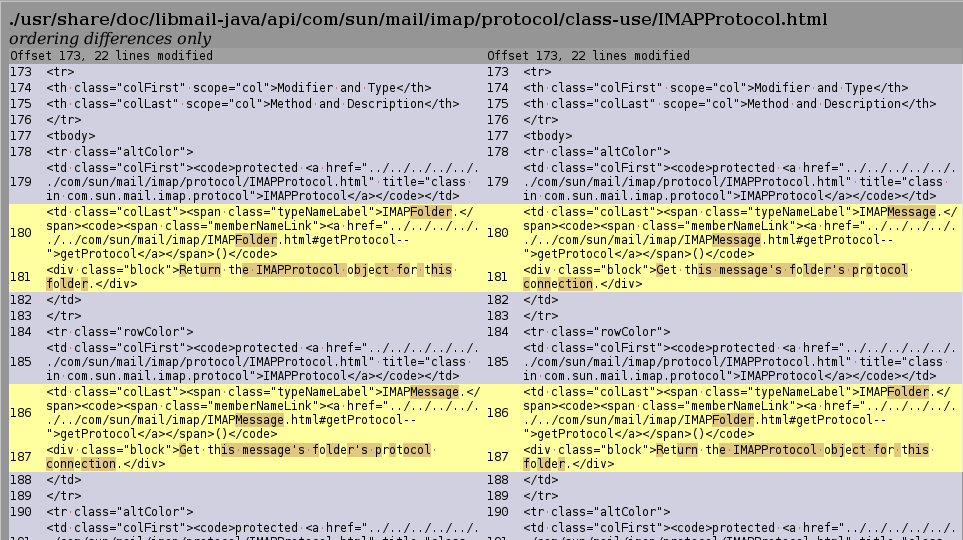
\includegraphics[width=0.95\textwidth]{fig/order-like-diff.png}
\caption{\label{fig:order}Comparison of two HTML files with ordering-only differences.}
\end{figure}

}
\section[Improved support for APK files]{Improved support for APK files}
\nopagebreak[4]{
Diffoscope compares APK files using \texttt{apktool}. This tool tries to disassemble the package back to
the project and resource files. The disassembled files are then compared using the suitable tool.

There was a number of improvements made for APK files comparison.
\begin{itemize}[noitemsep]
\item APK metadata, generated by \texttt{apktool} and written into the special file \path{apktool.yml}, is now handled separately from the rest of the files. 
It is renamed into ``APK metadata'' to reflect its contents; in addition, the APK file name itself is removed from the metadata, since the goal of diffoscope is to compare the contents of the file, regardless of their name.
\item APK files difference now includes information about APK file as archive: level of compression, access rights etc. 
This is done using \texttt{zipinfo}, since APK files are essentially a kind of ZIP archive files.
\item \path{AndroidManifest.xml}, a mandatory file for every Android package including the general 
information about it, has a better support now. Previously, these files were compared twice: once in their encoded form and once in the decoded plain text form generated by \texttt{apktool}. Now diffoscope tries to find the difference in the decoded \path{AndroidManifest.xml}, and falls back to the comparison of encoded ones only if the former approach does not reveal any differences.
\end{itemize}

Figure \ref{fig:apk} shows how the HTML output looks like when run over two APK files. The diffoscope version in use has the described features included.
\FloatBarrier

\begin{figure}
\centering
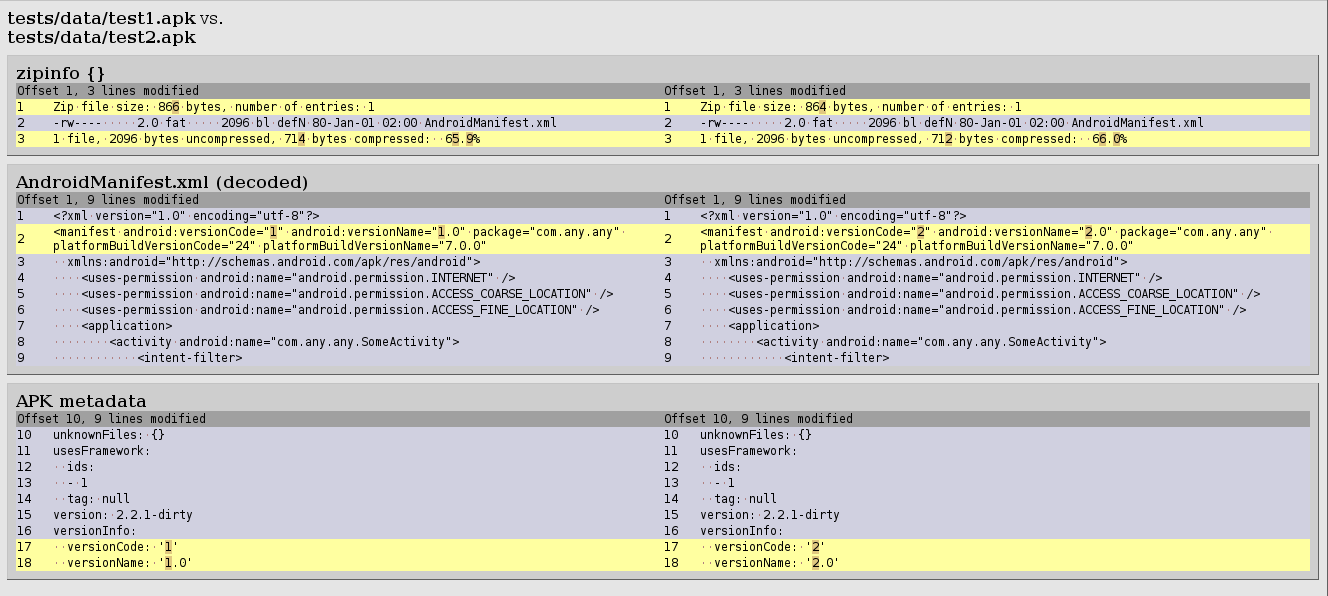
\includegraphics[width=0.95\textwidth]{fig/apk.png}
\caption{\label{fig:apk}Comparison of two APK files.}
\end{figure}

These changes are mostly useful for the F-Droid project \autocite{fdroid}, aiming to provide a collection of free Android applications. As part of the F-Droid project, the F-Droid Verification Server \autocite{fdroid-vfs} was set up, with all the applications being tested for reproducibility automatically.
Better support for APK files allows for a more informative diffoscope output provided for the application that fail these tests.


}
\section[Improved support for image files]{Improved support for image files}
\nopagebreak[4]{
Since diffoscope is mainly used to compare packages, support for the images is needed mainly for resource files used in some software. Currently, supported formats include JPEG, ICO, GIF and PNG.

The main approach to comparison of images at the moment involves converting them into ASCII-pseudographics using \texttt{libcaca} and comparing the resulting text. That approach allows for identifying issues related to content of the image, but some information -- such as palette, EXIF data, number of colors -- might be lost. Considering this, the new feature, comparison of image metadata, was added to diffoscope.\\
Metadata comparison is enabled for JPEG and ICO images. Information about the image is retrieved using \texttt{ImageMagick} tool.
The list of image properties extracted include e.g. image format, file size, height, width, orientation, compression type, compression quality, colorspace, number of channels. Information is extracted in text form and then compared using text comparison.

In addition, in cases where diffoscope is producing HTML output, it is possible to output images without converting them to text form. In these cases, generating ``visual difference'', image, showing the difference in the visual form, can result in a more informative output then pseudographics allows.
This behaviour was implemented in form of providing an additional field for the \texttt{Difference} objects, containing the visual difference images. These images are converted to \texttt{base64} form and embedded into the resulting HTML page using data URI protocol. Two types of visual difference are being generated for each pair of images at the moment:
\begin{itemize}[noitemsep]
  \item Pixel difference -- generated using \texttt{ImageMagick} \texttt{compare} tool. This kind of images underlines all the pixels that have different values for the compared images. This often includes differences which are not normally noticeable by human eye, such as compression artifacts.
  \item Flicker difference -- animation composed by alternating between the two images. Flicker difference is designed to provide a more human-perceptible way to view the difference, as it allows to notice the more significant changes between the two frames. 
\end{itemize}

Currently, the visual difference is computed only for the images of the same size and with only one frame per image, meaning this feature does not support comparing animated GIFs.
}

\section[Cross-container comparison]{Cross-container comparison}
\nopagebreak[4]{
The problem of comparing different types of archives was considered to be best solved by alerting fuzzy-matching module.
Diffoscope uses TLSH \autocite{oliver2013tlsh} library that implements fuzzy-matching using special hash values for files. 
By comparing hash values for different files, diffoscope is able to correctly recognize renamed files even when there is difference in the contents.\\\\
However, implementing the similar behaviour for containers was not a trivial task. 
If the container is considered a regular file and the hash is computed as for any other type of file, the result will be dependent on the type of the container, compression method, etc. Another option would be to compute the hash as combination of individual files' hashes. Unfortunately, that approach leads to unnecessary increase in computation time, since every container has to be extracted before finding the correspondence.\\\\
Even more important is the problem of comparing the nested containers. The most common use case is comparing compressed tarballs, e.g. \texttt{TAR.GZ} with \texttt{ZIP} archives. Both approaches described above would fail at this example, since not only the archive type, but the nesting level is different. However, both methods are quite common for software distribution, and it is desirable to have diffoscope compare their content, instead of stopping on the difference in the container type.\\\\
The proposed changes implement the following behaviour:
\begin{itemize}[noitemsep]
\item If both compared objects are containers, but have different types, they are compared by finding difference in:
\begin{itemize}[noitemsep]
\item Type of container
\item List of contents
\item Content
\end{itemize}
\item If one of the compared containers has one of following types: \texttt{gzip}, \texttt{bzip2}, \texttt{xz}, \texttt{dex}, it gets unpacked and the contents are compared. This can be safely done because all of these container types are guaranteed to have only one member. This way, the most common use case of nested containers is addressed.
\end{itemize}

Figure \ref{fig:containers} shows how the HTML output would look like for different types of containers with the proposed changes accepted. In this example, the types of containers, their list of content and the actual content of the files inside the containers differ between the two compared files.
\FloatBarrier

\begin{figure}
\centering
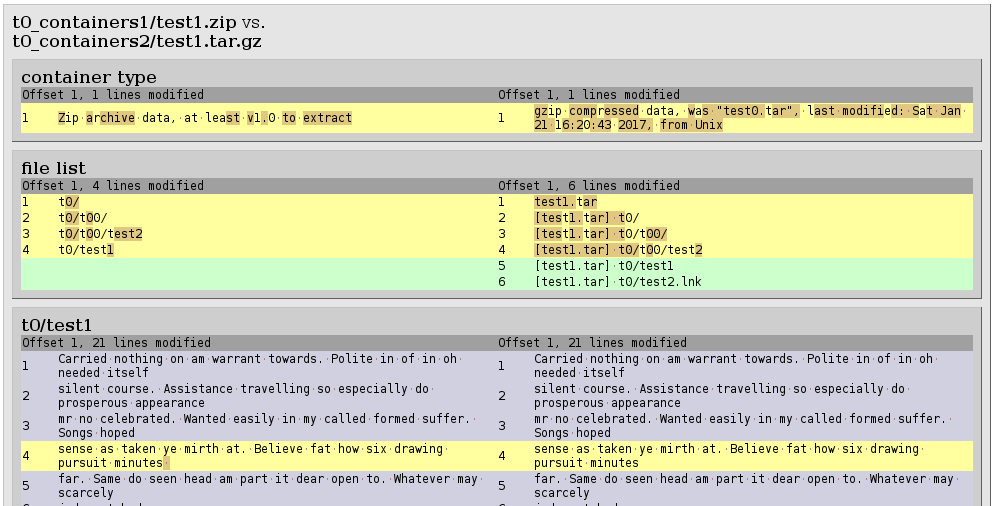
\includegraphics[width=0.95\textwidth]{fig/containers_new.png}
\caption{\label{fig:containers}Comparison of two containers.}
\end{figure}

The described changes for cross-container comparison are currently under review and therefore are not included in diffoscope yet.
}

%\cleardoublepage
 %New features
\section{Current state of the Reproducible Builds project}

\subsection[Debian]{Debian}
\nopagebreak[4]{
Debian continues its work toward ensuring that all of the packages in the distribution are bit-by-bit reproducible. 
To continuously check the status of reproducibility of individual packages, testing infrastructure is set up, reporting results on \autocite{tests-rbo}.
For the packages that are not reproducible for the tested variations, the diffoscope output is provided. That allows for an easier identification of underlying issues.\\\\
Currently, the work of Reproducible Builds project members within Debian is focused on three main areas:
\subsubsection[Continuous testing of Debian packages]{Continuous testing of Debian packages} 
Debian reproducibility testing server \autocite{tests-rbo} shows the status of reproducibility of Debian packages across several releases (stable, unstable, experimental) and architectures (amd64, i386, arm64, armhf). Reproducibility testing here means that the package is built two times, with some variations introduced between builds. For the packages that are not reproducible within this setup, diffoscope is run and its output is published, so it is easily accessible for package maintainers, Reproducible Builds project members and other interested parties. Reproducibility tests are re-run periodically, and the statistics about results of these tests is gathered.\\\\
Figure \ref{fig:stats_sid} shows the current status of reproducibility of Debian packages for unstable version of the distribution built for the amd64 target architecture. Note that the drop in number of reproducible packages in August, 2016 is connected to the new variation -- build path -- being introduced for unstable and experimental distribution. It turned out quite a lot of packages are affected by build path storing issue, and since then, there was quite a lot of work within a project targeting this issue.

\begin{figure}
\centering
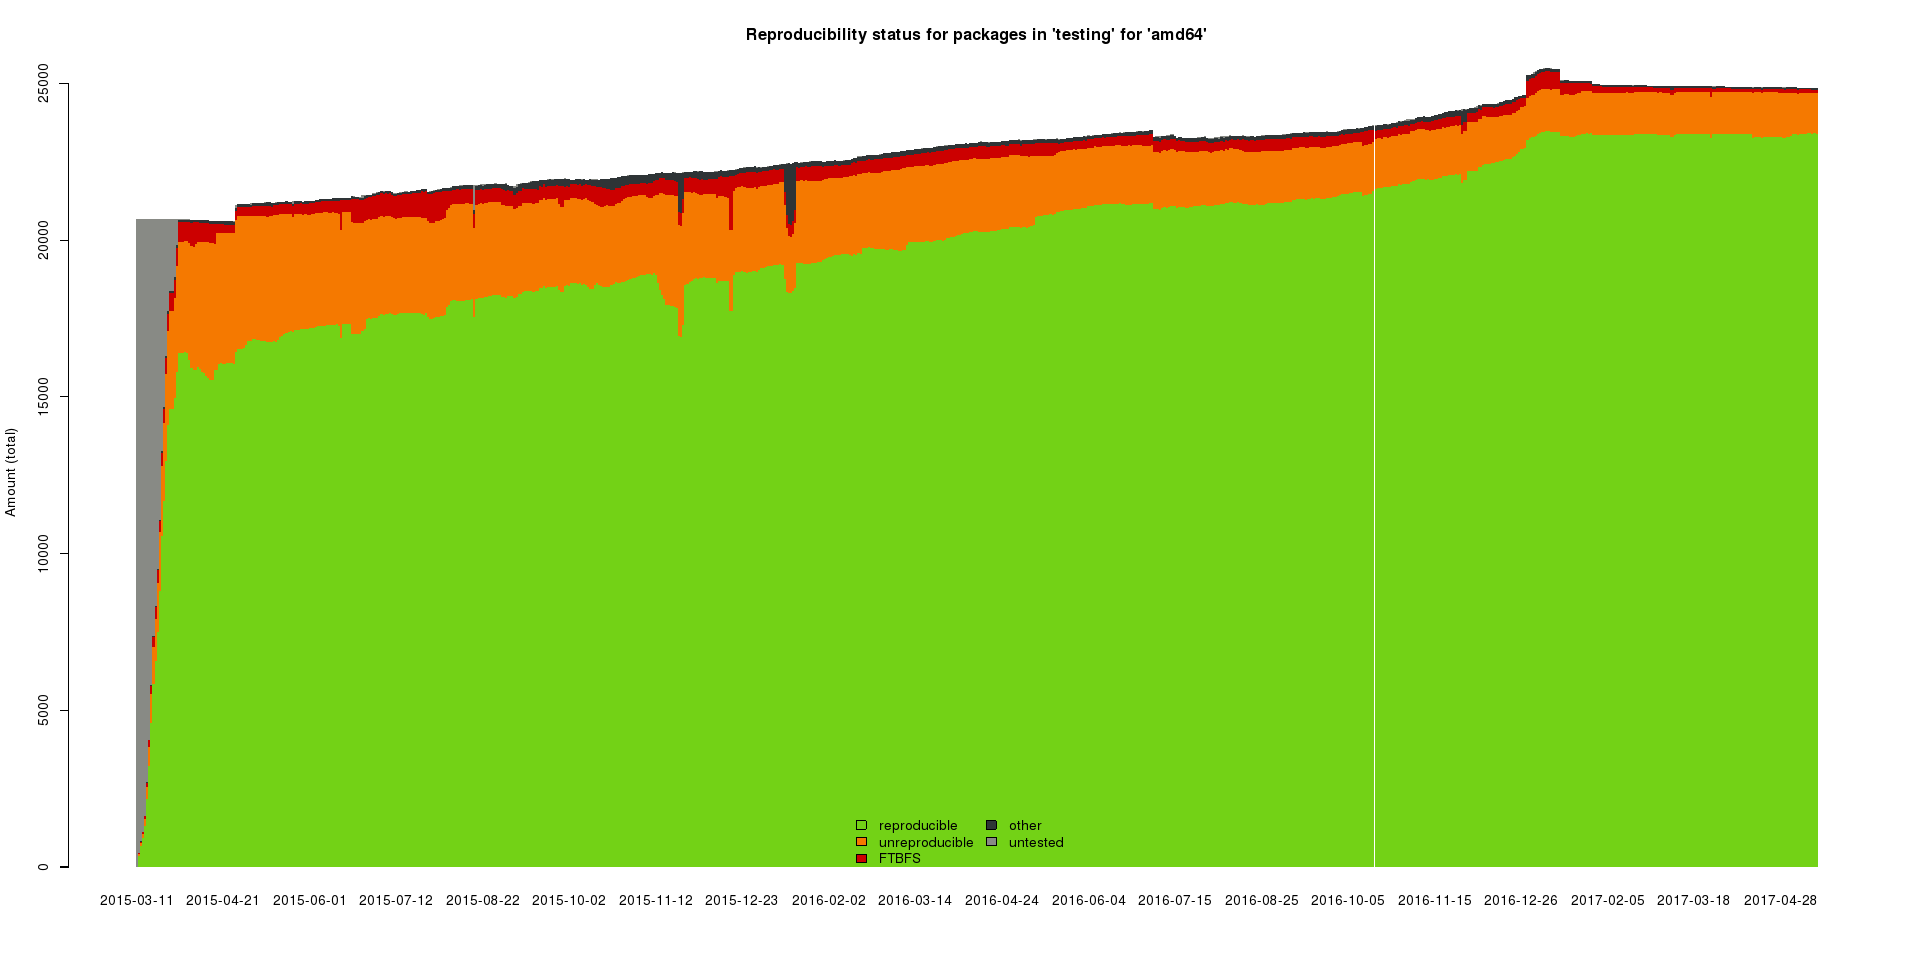
\includegraphics[width=0.95\textwidth]{fig/stats_pkg_state.png}
\caption{\label{fig:stats_sid}Overview of reproducible builds for packages in Debian unstable for amd64 architecture.}
\end{figure}

\subsubsection[Categorizing the issues]{Categorizing the issues} 
With diffoscope result for the packages available, Reproducible Builds project members try to identify the root issue causing reproducibility. It is often the case that the issue is not within the package itself, but rather in the tools used in the build process. Therefore, it is important to identify common issues and focus on resolving them in a unified way.\\\\
Some examples of the most common issues are:
\begin{itemize}[noitemsep]
\item \textit{Capturing build path} -- a lot of packages store the path where the package was built, during the build phase. This is inconvenient since this information is rarely helpful to end users; usually, the package is built on some dedicated build server and not on target computer. This issue is one of the main focus of Reproducible Build project members now, and they coordinate with maintainers of packages as well as build tools developers in order to address it.
\item \textit{Storing Timestamps} -- while this issue was addressed by \texttt{SOURCE\_DATE\_EPOCH}, some packages still record the build date or time.
\end{itemize}
Figure \ref{fig:stats_issues} illustrates the changes in the number of identified issues. This number generally rises over time, as new issues are being found and the old ones are often categorized into smaller and more specific issues. Even if the issue is completely dealt with, it is often left in records if it is believed information about it could be useful to other issues or other projects.\\\\

\begin{figure}
\centering
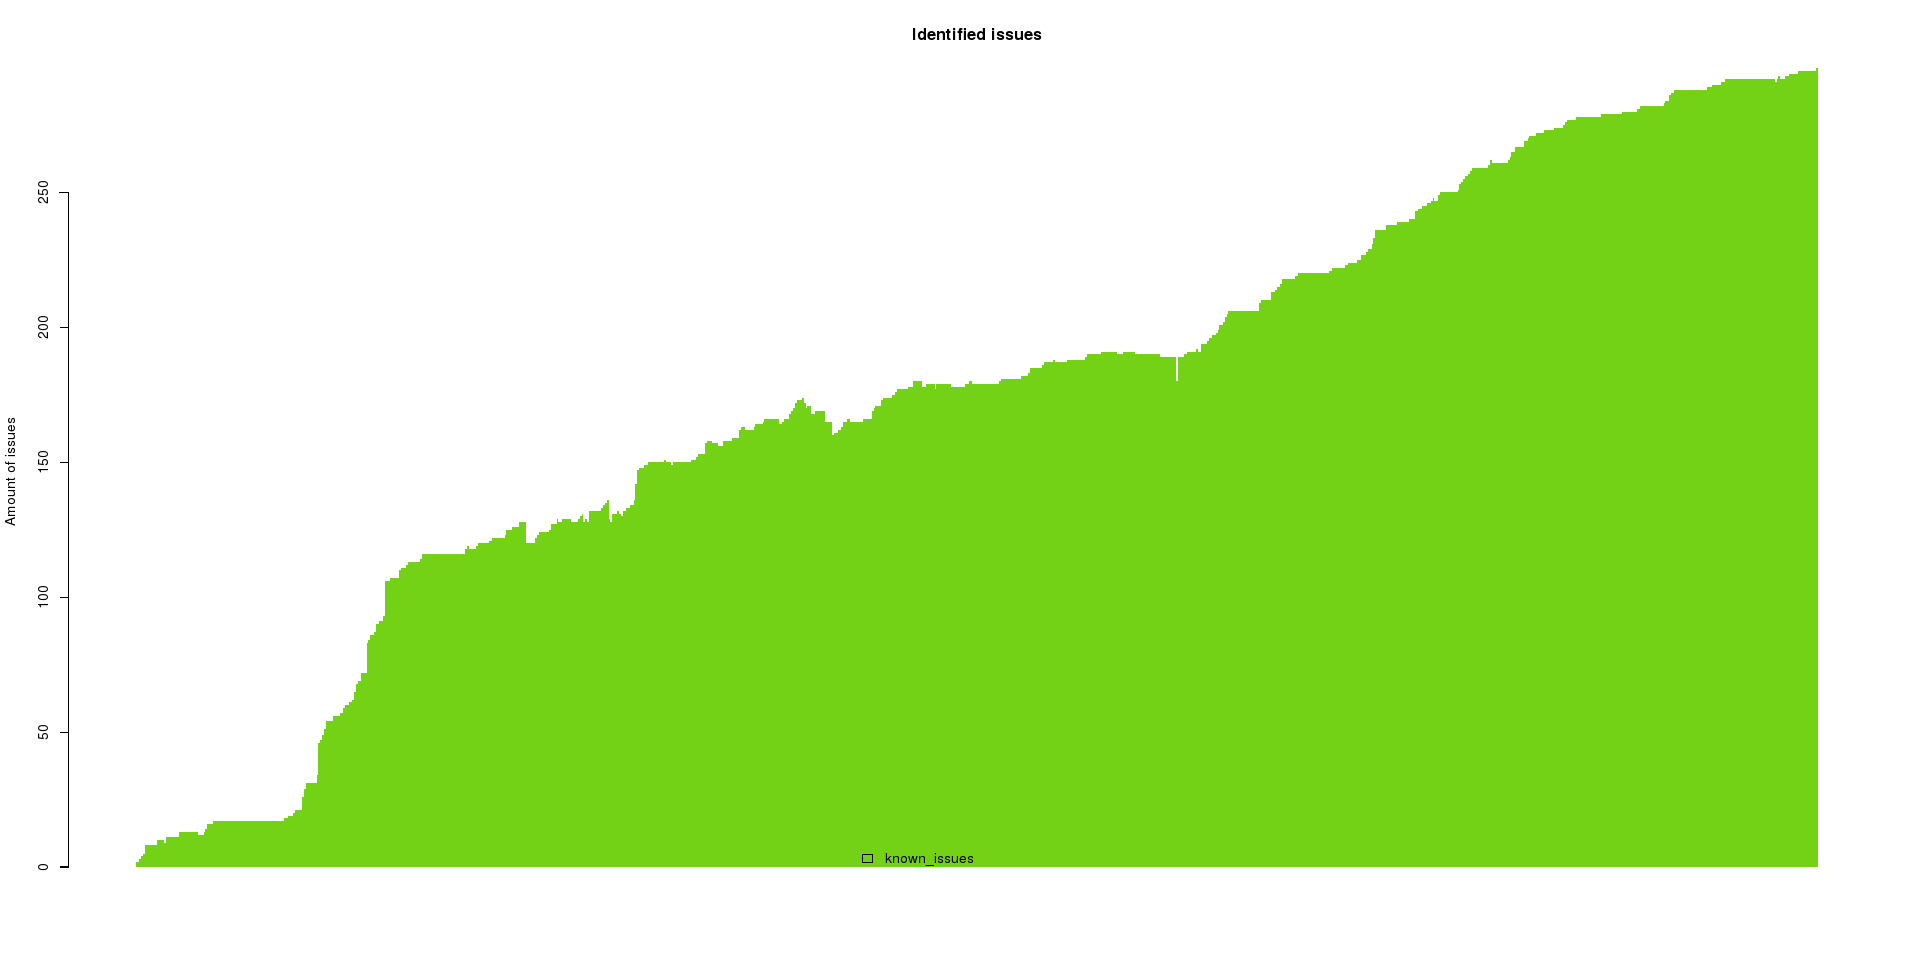
\includegraphics[width=0.95\textwidth]{fig/stats_issues.png}
\caption{\label{fig:stats_issues}Number of categorized reproducibility issues.}
\end{figure}

Figure \ref{fig:stats_notes} shows statistics about number of packages with notes attached to them, meaning that there is an identified issue or some sort of comment for them attached to them. Once again, a massive change is observed at around August, 2016, as the build path variation was introduced, resulting in a lot of packages being labeled with build path recording issue.\\

\begin{figure}
\centering
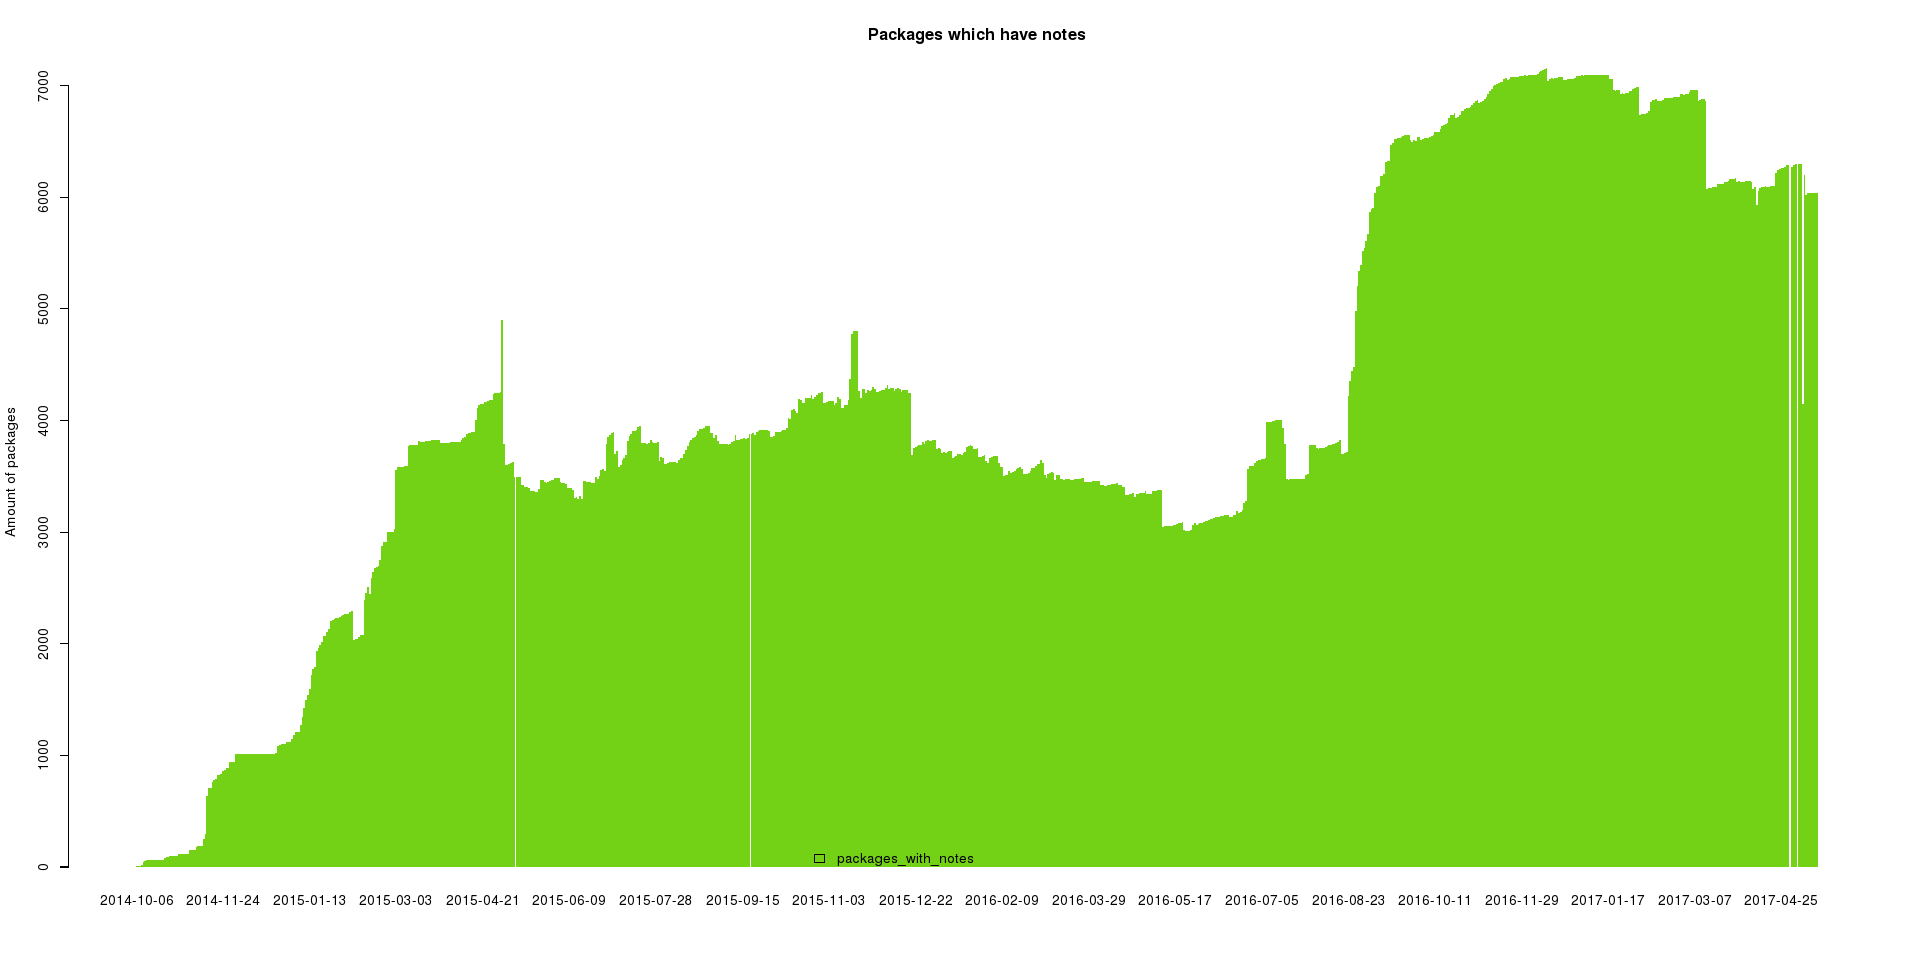
\includegraphics[width=0.95\textwidth]{fig/stats_notes.png}
\caption{\label{fig:stats_notes}Number of packages that have notes.}
\end{figure}
\subsubsection[Fixing reproducibility bugs]{Fixing reproducibility bugs}
While only package maintainers or developers actually have the means to fix their package, members of Reproducible Builds project try to help them by reporting the reproducibility issue. As a rule, they also provide a patch that is expected to fix the issue. Sometimes additional coordination with package maintainer or developer is required to ensure the patch fits well within the package and to clarify its meaning.\\\\
A lot of issues are related to the usage of the specific tool in the build process, and therefore it is usually preferred to focus on fixing these issues in the build tool in question, therefore helping all the packages using that tool to achieve reproducibility.

}
\subsection[F-droid]{F-droid}
\nopagebreak[4]{
The F-Droid project \autocite{fdroid}, that aims to provide an environment of free software for Android smartphones, has set up its own Verification Server \autocite{fdroid-vfs}. It functions in the similar fashion as Debian test infrastructure, rebuilding packages and providing the diffoscope output when results do not match.\\
}
\subsection[Other projects]{Other projects}
\nopagebreak[4]{
FreeBSD and NetBSD distributions also continue their work on reproducible builds. Currently, they use less variations between builds than Debian does, but within these constraint, they have achieved significant progress: NetBSD reported 100\% reproducibility within their build system in \autocite{netBSD} and FreeBSD is at 99.6\% at the moment \autocite{freeBSD}.
}


%\cleardoublepage
 %Current state of the project
\section{Conclusions}
\nopagebreak[4]{
  Reproducibility of software builds is important problem, critical for
  ensuring quality and security of open-source software. With the software
  building reproducibly, users can easily ensure no flaws were added to
  the product during build process and that the software indeed matches its
  source code. This problem attracted attention in various open-source projects,
  but outside of open-source world it is still not discussed enough. \\\\
  In this report, the history and motivation behind the
  Reproducible Builds project was presented. The definition of reproducibility
  in the software building process was given. An overview on the current reproducibility status of Debian operating system, as well as the steps taken to improve it, was discussed. Specifically discussed were the tools that the
  Reproducible Build project uses for testing reproducibility of software and
  identifying sources of unreproducibility. The particular tool for comparing
  two build outputs, named diffoscope, was discussed in detail, with emphasis on
  what can be done to improve it.
}

%\cleardoublepage
 %Conclusions

%\def\refname{what ever}% to change References title
%\addcontentsline{toc}{section}{References}%

\printbibliography


\end{document}
